
\chapter{Background}\label{cha:background}

Comordo Technologies is a startup in recommendation systems driven inside the bounds of LiU's incubator LEAD in Linköping and will in the future offer a cloud service for e-commerce. The base for the recommendation system is algorithms based on predication and machine learning. The company now stands to build a first version of it's recommendation system.

Comordo focuses on binary classification with implicit feedback such as generating recommendations for e-commerce using purchase history for users.

\Warning[TODO]{Write more!}

Needs to be able to actually run the algorithms, handle data and to automatically learn and optimize the algorithms and fit them to different types of data.

\Warning[TODO]{Rework paragraph}


\section{Use case}\label{sec:use}

\begin{enumerate}
    \item Purchase history and product data is provided by e-commerce clients and consumed.
    \item Load algorithms with purchase history and is run on a nightly basis.
    \item Repopulate recommendation database with new recommendations.
    \item Final customers visit the e-commerce website and are given recommendations delivered to the website via Commordo's remote API.
\end{enumerate}


\newpage
\section{System overview}\label{sec:sysoverview}

Figure \ref{fig:sysoverview} is a sketch of Commordo's recommender system, as planned for at the start of the thesis.

\begin{figure}[h!]
  \centering
    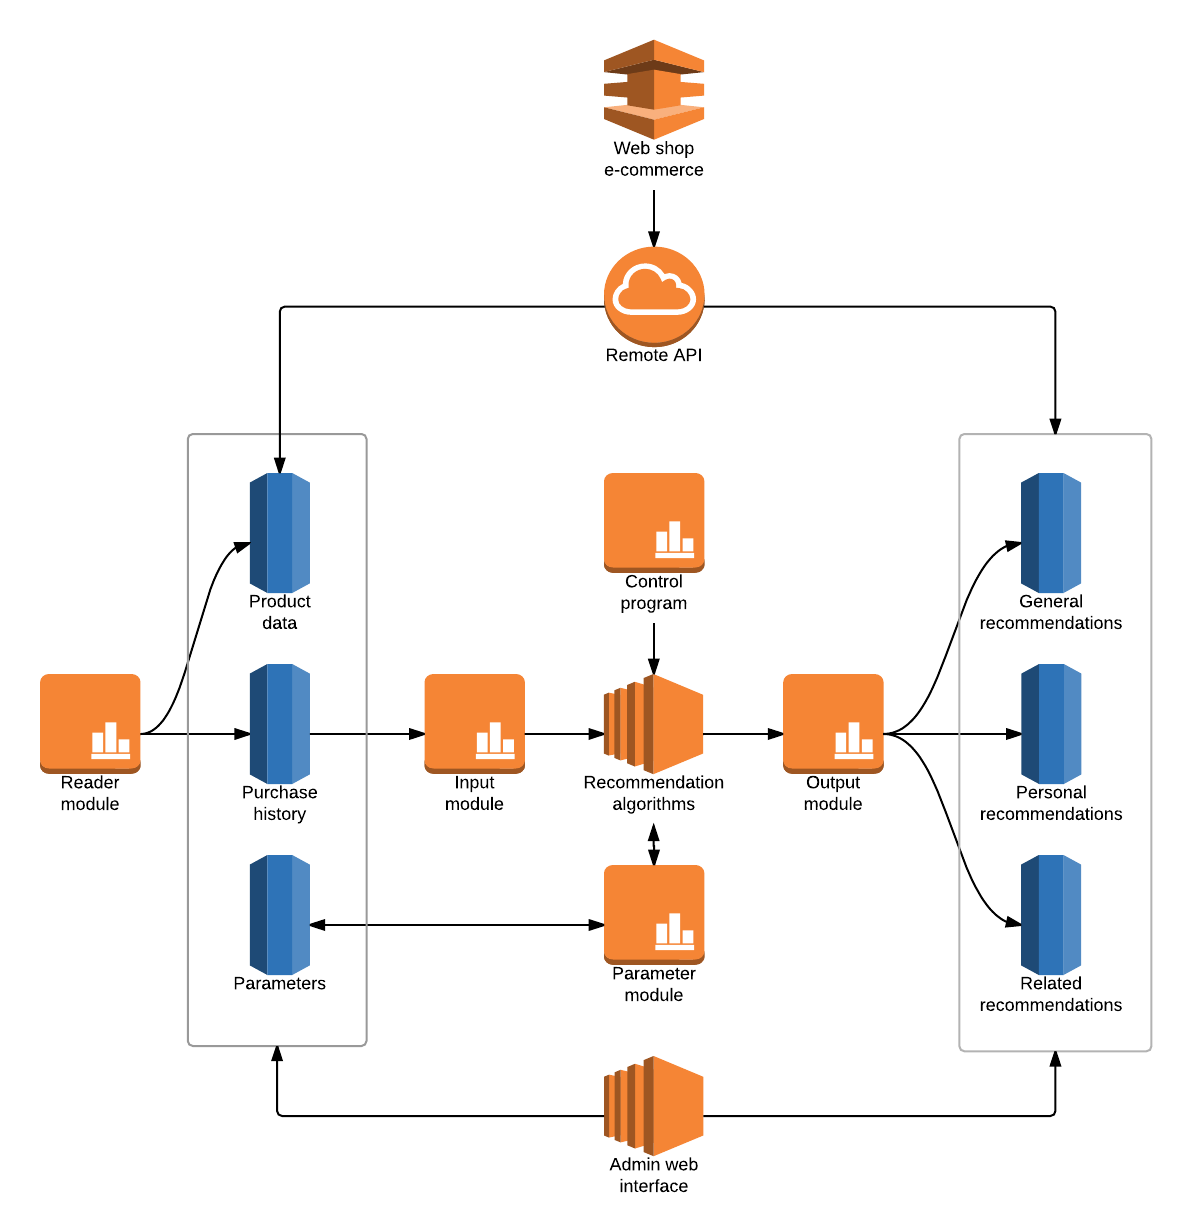
\includegraphics[width=0.9\textwidth]{fig/system_overview.png}
  \caption{Commordo's system sketch}
  \label{fig:sysoverview}
\end{figure}

\FloatBarrier

\begin{description}
    \item[Reader module] is responsible for reading data files provided by Commordo's clients.
    \item[Input module] provides the algorithms with transformed data.
    \item[Output module] populates the database with recommendations.
    \item[Control program] handles learning and optimization of the algorithms.
    \item[Parameter module] stores and adjusts parameters the algorithms use.
    \item[Remote API] is a REST based API, the endpoint for Commordo's clients.
\end{description}


\section{Task}\label{sec:task}

The task for this thesis is to complete the backend of Commordo's system. This includes the reader, input, output and parameter modules, the storage of purchase history and parameters and the control program. The other databases will be provided, but some level of adaptation might be needed. The admin interface and the remote API is not included in this thesis.

\Warning[TODO]{ Someothing more? Talk about questions here? Problem formulation? Or is this enough? }
